\documentclass[border=2mm]{standalone}
\usepackage{tikz}
\begin{document}
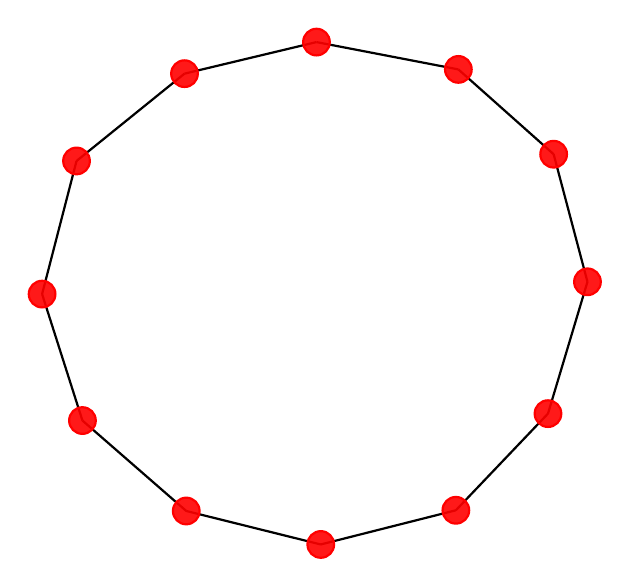
\begin{tikzpicture}[line width=0.5pt,fill opacity=0.9,scale = 3.5]
\tikzstyle{every path}=[draw, thick]
\tikzstyle{every node}=[draw, circle, fill=red, inner sep=3.4pt]
\coordinate (v_0) at (2.01100, -0.92432) {};
\coordinate (v_1) at (1.99540, 0.89822) {};
\coordinate (v_2) at (2.50114, -0.80030) {};
\coordinate (v_3) at (1.52300, -0.80287) {};
\coordinate (v_4) at (1.51664, 0.78369) {};
\coordinate (v_5) at (2.51020, 0.79910) {};
\coordinate (v_6) at (2.83533, -0.44968) {};
\coordinate (v_7) at (1.14643, -0.47477) {};
\coordinate (v_8) at (1.12491, 0.46695) {};
\coordinate (v_9) at (2.85586, 0.49143) {};
\coordinate (v_10) at (2.97854, 0.02858) {};
\coordinate (v_11) at (1.00000, -0.01602) {};
\path (v_0) -- (v_2);
\path (v_0) -- (v_3);
\path (v_1) -- (v_4);
\path (v_1) -- (v_5);
\path (v_2) -- (v_6);
\path (v_3) -- (v_7);
\path (v_4) -- (v_8);
\path (v_5) -- (v_9);
\path (v_6) -- (v_10);
\path (v_7) -- (v_11);
\path (v_8) -- (v_11);
\path (v_9) -- (v_10);
\node[red] (x_0) at (v_0) {};
\node[red] (x_1) at (v_1) {};
\node[red] (x_2) at (v_2) {};
\node[red] (x_3) at (v_3) {};
\node[red] (x_4) at (v_4) {};
\node[red] (x_5) at (v_5) {};
\node[red] (x_6) at (v_6) {};
\node[red] (x_7) at (v_7) {};
\node[red] (x_8) at (v_8) {};
\node[red] (x_9) at (v_9) {};
\node[red] (x_10) at (v_10) {};
\node[red] (x_11) at (v_11) {};
\end{tikzpicture}
\end{document}
